% Closed-loop form v1: what DRIVES the model during training, and why the residual form is
% the direct form. Answers the supervisor objection "the plant is nonlinear, so you cannot
% just subtract the difference in the controller output".
% Panel (a) is the loop that produced the data; the identity between the panels is the whole
% proof; panel (b) is what closed_loop_rollout actually runs.
% The grey region in (b) encloses exactly the part the identity uses, and it is linear.
% Style: figure-style.md, notation from jan-blockscheme-v4.
% Compile: pdflatex closed-loop-form-v1.tex
\documentclass[border=12pt]{standalone}
\usepackage{tikz}
\usetikzlibrary{arrows.meta, calc}
\usepackage{amsmath}

\begin{document}
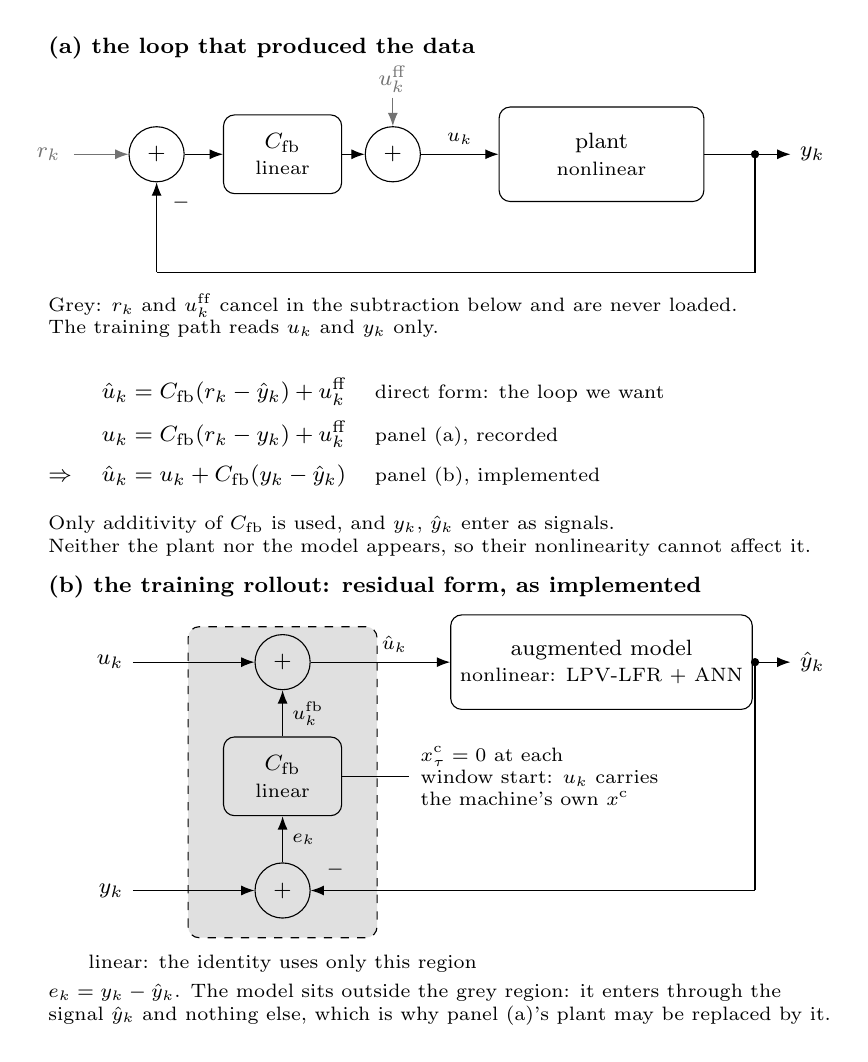
\begin{tikzpicture}[>=Latex, font=\footnotesize,
  block/.style={draw, rounded corners, minimum width=26mm, minimum height=12mm, align=center},
  rblock/.style={draw, rounded corners, minimum width=13mm, minimum height=11mm, align=center},
  small/.style={draw, rounded corners, minimum width=15mm, minimum height=10mm, align=center},
  sum/.style={draw, circle, minimum size=7mm, inner sep=0pt},
  jn/.style={circle, fill, minimum size=3pt, inner sep=0pt}]

% =================================================================================
% PANEL (a): the machine loop that produced the data
% =================================================================================
\node[anchor=west, font=\footnotesize\bfseries] at (-1.15,1.35)
  {(a) the loop that produced the data};

\node[sum]   (sa) at (0.35,0) {$+$};
\node[small] (ca) at (1.95,0) {$C_{\mathrm{fb}}$\\{\scriptsize linear}};
\node[sum]   (fa) at (3.35,0) {$+$};
\node[block] (pa) at (6.00,0) {plant\\{\scriptsize nonlinear}};

% reference and feedforward: present, and explicitly NOT part of the claim below
\node[black!55, left] at (-0.75,0) {$r_k$};
\draw[->, black!55] (-0.70,0) -- (sa.west);
\node[black!55] at (3.35,0.95) {$u^{\mathrm{ff}}_k$};
\draw[->, black!55] (3.35,0.72) -- (fa.north);

\draw[->] (sa.east) -- (ca.west);
\draw[->] (ca.east) -- (fa.west);
\draw[->] (fa.east) -- (pa.west) node[pos=0.50,above]{\scriptsize $u_k$};
\draw[->] (pa.east) -- (8.40,0);
\node[right] at (8.40,0) {$y_k$};
\node[jn] at (7.95,0) {};
\draw[-]  (7.95,0) -- (7.95,-1.50) -- (0.35,-1.50);
\draw[->] (0.35,-1.50) -- (sa.south);
\node[font=\scriptsize] at (0.66,-0.62) {$-$};

\node[anchor=west, align=left, font=\scriptsize] at (-1.15,-2.05)
  {Grey: $r_k$ and $u^{\mathrm{ff}}_k$ cancel in the subtraction below and are never loaded.\\
   The training path reads $u_k$ and $y_k$ only.};

% =================================================================================
% THE IDENTITY: this is the proof
% =================================================================================
\node[anchor=west, align=left, font=\footnotesize] at (-1.15,-3.55)
  {$\begin{aligned}
      \hat u_k &= C_{\mathrm{fb}}(r_k-\hat y_k) + u^{\mathrm{ff}}_k
        && \text{\scriptsize direct form: the loop we want} \\[1pt]
      u_k &= C_{\mathrm{fb}}(r_k-y_k) + u^{\mathrm{ff}}_k
        && \text{\scriptsize panel (a), recorded} \\[2pt]
      \Rightarrow\quad \hat u_k &= u_k + C_{\mathrm{fb}}(y_k-\hat y_k)
        && \text{\scriptsize panel (b), implemented}
   \end{aligned}$};

\node[anchor=west, align=left, font=\scriptsize] at (-1.15,-4.85)
  {Only additivity of $C_{\mathrm{fb}}$ is used, and $y_k$, $\hat y_k$ enter as signals.\\
   Neither the plant nor the model appears, so their nonlinearity cannot affect it.};

% =================================================================================
% PANEL (b): the training rollout, residual form
% =================================================================================
\node[anchor=west, font=\footnotesize\bfseries] at (-1.15,-5.50)
  {(b) the training rollout: residual form, as implemented};

% the linear region, drawn first so it sits behind the nodes
\fill[black!12, rounded corners] (0.75,-9.95) rectangle (3.15,-6.00);
\draw[dashed, rounded corners] (0.75,-9.95) rectangle (3.15,-6.00);

\node[sum]   (us) at (1.95,-6.45) {$+$};
\node[small] (cc) at (1.95,-7.90) {$C_{\mathrm{fb}}$\\{\scriptsize linear}};
\node[sum]   (ec) at (1.95,-9.35) {$+$};
\node[block] (mc) at (6.00,-6.45) {augmented model\\{\scriptsize nonlinear: LPV-LFR $+$ ANN}};

\draw[->] (0.05,-6.45) -- (us.west);
\node[left] at (0.05,-6.45) {$u_k$};
\draw[->] (0.05,-9.35) -- (ec.west);
\node[left] at (0.05,-9.35) {$y_k$};

\draw[->] (ec.north) -- (cc.south) node[pos=0.5,right]{\scriptsize $e_k$};
\draw[->] (cc.north) -- (us.south) node[pos=0.5,right]{\scriptsize $u^{\mathrm{fb}}_k$};
\draw[->] (us.east) -- (mc.west) node[pos=0.60,above]{\scriptsize $\hat u_k$};
\draw[->] (mc.east) -- (8.40,-6.45);
\node[right] at (8.40,-6.45) {$\hat y_k$};
\node[jn] at (7.95,-6.45) {};
\draw[-]  (7.95,-6.45) -- (7.95,-9.35);
\draw[->] (7.95,-9.35) -- (ec.east);
\node[font=\scriptsize] at (2.62,-9.08) {$-$};

% controller initial condition, the second question this figure answers
\draw[thin] (cc.east) -- (3.55,-7.90);
\node[anchor=west, align=left, font=\scriptsize] at (3.58,-7.90)
  {$x^{\mathrm{c}}_{\tau}=0$ at each\\
   window start: $u_k$ carries\\
   the machine's own $x^{\mathrm{c}}$};

\node[anchor=north, font=\scriptsize] at (1.95,-10.05)
  {linear: the identity uses only this region};

\node[anchor=west, align=left, font=\scriptsize] at (-1.15,-10.80)
  {$e_k=y_k-\hat y_k$. The model sits outside the grey region: it enters through the\\
   signal $\hat y_k$ and nothing else, which is why panel (a)'s plant may be replaced by it.};

\end{tikzpicture}
\end{document}
